\documentclass[letterpaper,10pt]{article}

\usepackage{titling}
\usepackage{listings}
\usepackage{url}
\usepackage{setspace}
\usepackage{subfig}
\usepackage{sectsty}
\usepackage{pdfpages}
\usepackage{colortbl}
\usepackage{multirow}
\usepackage{multicol}
\usepackage{relsize}
\usepackage{amsmath}
\usepackage{wasysym}
\usepackage{fancyvrb}
\usepackage{amssymb}
\usepackage{ifsym}
\usepackage{amsmath,amssymb,amsthm,graphicx,xspace}
\usepackage[titlenotnumbered,noend,noline]{algorithm2e}
\usepackage[compact]{titlesec}
\usepackage{XCharter}
\usepackage[T1]{fontenc}
\usepackage{tikz}
\usetikzlibrary{arrows,automata,shapes,trees,matrix,chains,scopes,positioning,calc}
\tikzstyle{block} = [rectangle, draw, fill=blue!20, 
    text width=2.5em, text centered, rounded corners, minimum height=2em]
\tikzstyle{bw} = [rectangle, draw, fill=blue!20, 
    text width=4em, text centered, rounded corners, minimum height=2em]

\definecolor{namerow}{cmyk}{.40,.40,.40,.40}
\definecolor{namecol}{cmyk}{.40,.40,.40,.40}

\let\LaTeXtitle\title
\renewcommand{\title}[1]{\LaTeXtitle{\textsf{#1}}}


\newcommand{\handout}[5]{
  \noindent
  \begin{center}
  \framebox{
    \vbox{
      \hbox to 5.78in { {\bf ECE356: Database Systems } \hfill #2 }
      \vspace{4mm}
      \hbox to 5.78in { {\Large \hfill #4  \hfill} }
      \vspace{2mm}
      \hbox to 5.78in { {\em #3 \hfill} }
    }
  }
  \end{center}
  \vspace*{4mm}
}

\newcommand{\lecture}[3]{\handout{#1}{#2}{#3}{Lecture #1}}
\newcommand{\tuple}[1]{\ensuremath{\left\langle #1 \right\rangle}\xspace}

\addtolength{\oddsidemargin}{-1.000in}
\addtolength{\evensidemargin}{-0.500in}
\addtolength{\textwidth}{2.0in}
\addtolength{\topmargin}{-1.000in}
\addtolength{\textheight}{1.75in}
\addtolength{\parskip}{\baselineskip}
\setlength{\parindent}{0in}
\renewcommand{\baselinestretch}{1.5}
\newcommand{\term}{Winter 2018}

\singlespace


\begin{document}

\lecture{ 16 --- Query Processing, Continued }{\term}{Jeff Zarnett}

\section*{Query Processing, Continued}

Having examined in some detail the idea of different strategies for carrying out a select operation. The next thing we would like to do is expand to more advanced queries, specifically, join queries. Join queries will be cripplingly inefficient if they operate on unsorted data. Remember that in a join, we need to match a tuple of the left hand relation with a tuple of the right hand relation. If for every tuple we had to linearly search the right hand relation, that would be painful. One way or another, we probably have to sort one of the relations to make this work.

\subsection*{Digression: Sorting}

So let us take a few minutes to talk about sorting. Wait, I hear you say, you already know ALL about sorting, insertion sort and selection sort and bogo sort and radix sort. Yes, also merge sort and quick sort. When you learn about sorting in a data structures and algorithms context, you are sorting a manageable amount of data. Manageable in the previous sentence means the full set of data can be fit into memory. For those, we can use all the standard algorithms. In the world of databases we need an algorithm that does not depend on loading everything into memory.

Sorting relations that do not fit into memory is called external sorting, and we will learn the external sort-merge algorithm from~\cite{dsc}. The basic plan works a lot like the merge sort algorithm works: divide the data into smaller units, sort the smaller units, then merge the smaller sorted units into a larger sorted unit. The sorting of each smaller unit will take place in memory, as per normal, and then we need to do an N-way merge where $N$ is the number of smaller units to be merged. Let's expand on this.

Step one of the algorithm is to divide the file into $N$ chunks of size $M$ where $M$ is the number of blocks that can fit into the area of memory available for sorting. Each chunk is as big as it can be for the constraints of the system, but no bigger. This chunk is called a \textit{run}. Each run $i$ is then sorted and it is written to a temporary file called $R_{i}$.

Step two of the algorithm now merges it. If $N$ is less than $M-1$ we have the simpler case and we can complete the merge in one pass. In that case we load the first block of $R_{i}$ for each $i$ from $0$ to $N-1$ into memory and we allocate an output block. Then we choose the first tuple from the all of the blocks, and move it into the output block. If a block $R_{i}$ becomes empty, replace it with the next block in that run (if there is one). If the output block becomes full, write it out and allocate a new output block. Continue this algorithm until all runs are empty. 

If $N$ is large enough that we cannot do it all in a single pass, we will do multiple passes. We will combine the first $M-1$ runs into a temporary file, and then the next (up to) $M-1$ runs, and so on, until the last run has been processed. Then we repeat the process using the larger runs as input until we produce the sorted file.

An example may help to clarify. Suppose the file consists of 10~000 blocks and we can fit 50 blocks in memory to do the sort. We can therefore create runs of 10~000/50 = 200 blocks each. Each run is sorted. Then we come to merge them. We cannot fit a block from each of the 200 runs inside the 49 available (50 - 1 block for output) so we must do multiple passes. The first pass sorts runs 1 through 49 into a new run (let's call it $R'_{1}$, then runs 50 - 98 into $R'_{2}$, et cetera, until the last one which is then 197-200 in $R'_{5}$. These larger $R'$ runs are then combined using the same merge procedure as before. Since there are only 5 we are sure the merge will complete in this second pass and we have the output file we wanted.

A visual representation of a two step sort merge from~\cite{dsc}:

\begin{center}
	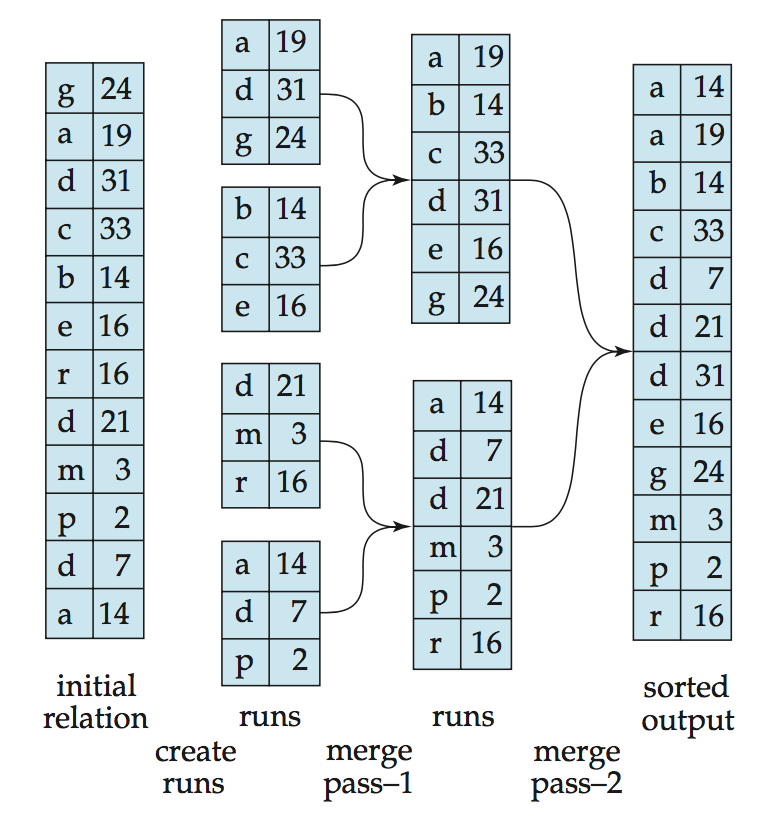
\includegraphics[width=0.5\textwidth]{images/external-merge}
\end{center}

Sorting has a cost, of course. 

\bibliographystyle{alphaurl}
\bibliography{356}


\end{document}
